% !TEX root = ../thesis-index.tex


\chapter{Briding mean field and finite width analysis}\label{ch:bn_MF}


There is a growing demand for a theoretical understanding of neural networks to improve their safety, robustness, computational and statistical effectiveness. Originating in statistical mechanics for investigating complex systems with interacting particles, this theory has been repurposed in recent years for exploring neural network dynamics under the regime of infinite width. By going beyond the microscopic changes of individual neurons, mean field analysis has revealed the collective neuronal behaviors that emerge at initialization~\cite{pennington2018emergence,yang2018a,pennington2017nonlinear}, throughout training \cite{jacot2018neural,bach2021gradient,lee2019wide}, and after training \cite{chizat2020implicit,ba2019generalization}.

In this chapter, we delve into the role of mean field theory at initialization when network weights are allocated randomly. Pioneering works by~\citet{pmlrv9glorot10a} and~\citet{saxe2013exact} underscored the impact of initialization on training, paving the way for mean field theory to uncover a wealth of insights. Examples include identifying connections between wide neural networks and Gaussian processes~\cite{neal2012bayesian,matthews2018gaussian,jacot2018neural}, examining the concentration of singular values of input-output Jacobians~\cite{pennington2018emergence,feng2022rank}, and designing activation functions~\cite{klambauer2017self,ramachandran2017searching,li2022neural}. Remarkably,~\citet{xiao2018dynamical} introduced an initialization scheme capable of training convolutional networks comprising $10000$ layers.

A common thread among these studies is the dynamics of inner products between hidden representations, encoded in their Gram matrix. Mean field theory models these dynamics via a difference equation derived from the infinite-width limit of the network. However, mean field analysis is inherently prone to approximation errors when dealing with networks of finite width. As \citet{matthews2018gaussian} observed, this error grows with depth, ultimately leading to vacuous error bounds in the infinite depth limit. To tackle this issue,  they propose to increase the network width proportional to depth. This idea is echoed in other studies which propose maintaining a constant ratio between depth and width~\cite{hanin2019finite,li2021future}, a regime in which~\citet{hanin2022correlation} confirmed a constant concentration bound for mean field estimates.

Can we achieve a bounded mean field error when the width is finite? We answer this question affirmatively for MLPs that are endowed with batch normalization. In particular, we show that under some technical assumption on the underlying dynamics (as formally expressed in Theorem~\ref{MF:thm:concentration}), the mean field estimation error for Gram matrices remains bounded at infinite depth. Specifically, we demonstrate that this error is limited by $\text{width}^{-1/2}$ with high probability. This contrasts with the vacuous concentration bounds at infinite depth observed in the absence of normalization~\cite{li2022neural}. Our results highlight the importance of existing mean field analyses of batch normalization by~\citet{yang2018a}, and demonstrate their high accuracy in the finite width scenarios that are relevant for practical applications.\footnote{Codes available at \url{https://github.com/ajoudaki/mean field-normalization}.}


\section{Related works}
Numerous studies~\cite{saxe2013exact,feng2022rank,yang2018a} have provided valuable insights into training neural networks by studying input-output Jacobians of neural networks with and without normalization at initialization. For example, ~\citet{feng2022rank} have shown that the rank of the input-output Jacobian of neural networks without normalization at initialization diminishes exponentially with depth, while ~\citet{yang2018a} have shown that batch normalization avoids this exponential diminishing. 

The spectrum of Jacobians is intimately related to the spectra of Gram matrices. 
A Gram matrix (G-matrix) contains inner products of samples within a batch (\eqref{MF:eq:gram_matrix}). Thus, a degenerate G-matrix for the penultimate layer implies that the outputs are insensitive to the inputs~\cite{feng2022rank,li2022neural}.  
Rank collapse in the last hidden layer occurs in various neural network architectures, including MLPs~\cite{saxe2013exact}, convolutional networks~\cite{daneshmand2020batch}, and transformers~\cite{dong2021attention}, and leads to ill-conditioning of the input-output Jacobian, which slows training~\cite{daneshmand2021batch,pennington2018emergence,yang2018a}. ~\citet{saxe2013exact} have shown that avoiding rank collapse can accelerate the training of deep linear networks, making it a focus of theoretical and experimental research~\cite{pennington2018emergence,daneshmand2020batch,daneshmand2021batch}.


A recent line of research~\cite{daneshmand2020batch} postulates that batch normalization can enhance the training of deep neural nets by avoiding the rank collapse. This claim has been supported by empirical evidence~\cite{yang2018a,daneshmand2020batch}, as well as theoretical studies for neural networks with infinite widths~\cite{yang2018a} and linear activation~\cite{daneshmand2021batch}. It has been shown that batch normalization prevents degenerate representations at initialization~\cite{daneshmand2020batch}, and orthogonalizes representations~\cite{daneshmand2021batch}. However, these results are limited to linear activations.
The present study extends these findings to neural networks with finite widths and non-linear activations, under an assumption from Markov chain theory. 


\section{Problem settings and background}

\paragraph{Notation and terminology.}
$I_n$ denotes the identity matrix of size $n\times n$ and $1_n$ denotes the all ones vector in $\R^n$.  
$\otimes$ refers to Kronecker product. $\mu_X$ refers to the probability measure of the random variable $X$. We use $f\lesssim g, g \gtrsim f$ and $f = \O(g)$ to denote the existence of an absolute constant $c$ such that $f\le c\; g.$ 
$\norm{v}$ for a vector $v$ denotes the $L^2$ norm.
$\norm{C}$ for matrix $C$ denotes the $L^2$ operator norm $\norm{C}=\sup_{x\in\R^n}\norm{C x}/\norm{x}$, $\norm{C}_F$ denotes the Frobenius norm. We use $\kappa(C)$ to denote the ratio of largest to smallest eigenvalue. Both $h_{r\cdot}$ and $\row_r(h)$ denote row-vector representation of the $r$-th row of $h.$ Finally, $X\sim \Normal(\mu,\sigma^2)^{n\times m}$ denotes $X\in\R^{n\times m}$ is a Gaussian matrix whose elements are drawn \iid from $\Normal(\mu,\sigma^2).$ 

\paragraph{Setup.}
Let $h_\ell\in \R^{d\times n}$ denote the hidden representation at layer $\ell$, where $n$ corresponds to the size of the mini-batch, and $d$ denotes the width of the network that is kept constant across all layers. The sequence  $\{h_\ell\}$ is a Markov chain as
\begin{align}\label{MF:eq:chain}
h_{\ell+1}:=W_\ell \act\circ\BN(h_\ell), && W_\ell\sim\Normal(0,\nfrac1d)^{d\times d},
\end{align}
where $h_0\in\R^{d\times n}$ is the input batch, $\act$ is the element-wise activation function, and $\BN$ is the batch normalization \cite{ioffe2015batch}, which applies row-wise centering and scaling by standard deviation:
\begin{align*}
\BN(x) = \frac{x - \text{mean}(x)}{\sqrt{\text{Var}(x)}}, && \forall r: \row_r(\BN(h)) = \BN(\row_r(h)).
\end{align*} 
  

\section{Mean field models and fixed-point analyses}
\subsection{Mean field Gram dynamics}
The Gram matrix $G_\ell$ is defined as the matrix of inner products of hidden representations at layer $\ell$ as seen in the equation below:
\begin{align}\label{MF:eq:gram_matrix}
G_\ell := \frac1d (\act\circ\BN(h_\ell))(\act\circ\BN(h_\ell))^{\top}.
\end{align}
Understanding the dynamics of $G_\ell$ is a significant challenge in deep learning theory, and has been the subject of several studies \cite{yang2018a,pennington2018emergence,pennington2017nonlinear}. Due to the randomness of weights, determining the trajectory of this random process proves to be arduous. By tending width $d$ to infinity, i.e., the mean field regime, we can approximate these stochastic dynamics with a deterministic dynamics as below:
\begin{align}\label{MF:eq:MF_recurrence}
\overline{G}_{\ell+1} = \E_{h\sim \Normal(0,\overline{G}_\ell)}\left[\act\left(\frac{ \sqrt{n} M h}{\| Mh\|}\right)^{\otimes 2}\right],
\end{align}
Where $\overline{G}_{0} = G_0$ serves as the input G-matrix and ${M = I_n - \frac1n1_n^{\otimes 2}}$ applies mean reduction on the preactivations. The mean field approach in this context assists in elucidating the analysis of Gram matrices.

\subsection{Fixed point analysis for infinitely deep and wide Networks}
The fixed points of the mean field dynamics, as expressed in ~\eqref{MF:eq:MF_recurrence} may help elucidate the properties of $\overline{G}_{\ell}$ as $\ell \to \infty$. 
\citet{yang2018a} provide a comprehensive characterization of these fixed-points, denoted by $\C$, for neural networks with batch normalization. For networks with linear activations, \citet{yang2018a} establish a global convergence to these well-conditioned fixed-points. While they empirically observe convergence to these well-conditioned fixed-point for networks with non-linear activations, that is not established theoretically. In other words, it is challenging to describe the properties of $\overline{G}_\ell$ for finite width and depth, and it is unclear how the fixed-point Gram matrix $\C$ can inform us about~$G_\ell$.

\subsection{An observation}
Through an empirical observation we can demonstrate that $\C$ may not always provide an accurate estimate for $G_\ell$. We observe that for a network without batch normalization and linear activations (when $\act\circ\BN=identity$ in~\eqref{MF:eq:chain}), the Frobenius distance between $G_\ell$ and $\C$ increases with $\ell$. In contrast, $G_\ell$ converges to a neighborhood of $\C$ when the network includes batch normalization layers. These observations suggest that the mean field estimate $\C$ from \citet{yang2018a} accurately represents $G_\ell$ when batch normalization is present.
  

 
\begin{figure}
    \centering
    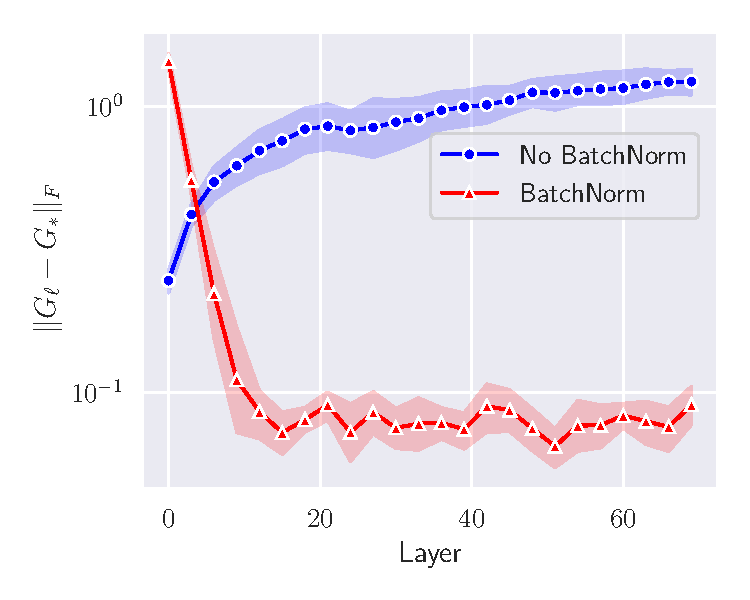
\includegraphics[width=0.45\textwidth]{figures/bn_without.pdf}
    \vspace{-.5cm}
    \caption{\textit{Mean field error amplification with(out) batch-normalization.} The horizontal axis represents the number of layers $\ell$ (linear), while the vertical axis (log-scale) shows $\|G_\ell- G_*\|_F$, for networks with $n=5, d=1000$. The traces show mean and shades indicate $90\%$ confidence intervals over $10$ independent simulations. }
    \label{MF:fig:rapidly_mixing}
\end{figure}



\subsection{The challenge of depth for mean field theory}
Mean field analysis suffers from a systematic estimation error that increases with depth. Assuming that $\overline{G}_0= G_0$, then an error of $O(d^{-1/2})$ is observed between $\overline{G}_1$ and $G_1$ due to the concentration of empirical covariance. Consequently, the mean field dynamics in \eqref{MF:eq:MF_recurrence} incur an error of $O(d^{-1/2})$ at each layer~\cite{li2022neural}. As depth $\ell$ grows, these errors are amplified, and the bounds on $\| G_\ell - \overline{G}_\ell\|_F $ become vacuous, thus raising questions about the practical applicability of these fixed-point analyses when width is finite. 

Several studies strive to refine the mean field model to enhance its predictive accuracy ~\cite{matthews2018gaussian,hanin2019finite,li2022neural}. \citet{li2022neural} propose using a stochastic differential equation to model the layer-wise $O(d^{-1/2})$ estimation error for mean field Gram dynamics. This approach allows for accurate predictions of Gram dynamics for MLPs with activation functions but only in the infinite-width-and-depth regime. Our observations, however, suggest that for networks with batch normalization, the deterministic model of Gram matrices provides a surprisingly accurate estimate.

\citet{daneshmand2021batch} established this observation for multilayer perceptrons (MLPs) with batch normalization (BN) and linear activations, subject to specific conditions. They demonstrated that as $\ell$ increases, batch normalization progressively aligns the Gram matrices $G_\ell$ with the identity matrix, which coincides with $G_*$ for such networks \cite{yang2018a}. \citet{yang2018a} further proved a concentration bound for $\|G_\ell - G_*\|_F$ in networks with batch normalization and linear activations. However, both these findings are limited to linear activations. Our objective is to extend these results to networks incorporating non-linear activations.




\section{Concentration bounds for Mean field Predictions with Batch Normalization}


\subsection{Geometric ergodic assumption} 
The chain of hidden representations obeys a non-linear stochastic recurrence. Despite this non-linearity, the distribution associated with the representation obeys a linear fixed-point iteration determined by the Markov kernel $K$ associated with the chain $h_\ell$. The distribution of $h_\ell$, denoted by $\mu_{\ell},$ obeys 
\begin{align} \label{MF:eq:dist_recurrence}
    \mu_{\ell+1} = T(\mu_{\ell}), \quad T(\mu) := \int K(x,y) d\mu(y).
\end{align}
The fixed-points of the above equation are invariant distributions of the chain, which we denote by $\mu_*$.  Recall that the total variation for distributions over $d\times n$ matrices can be defined as $\tv{X}{Y}:=\sup_{A\subseteq\R^{d\times n}} |\mu_X(A)-\mu_Y(A)|.$
Notably, the above recurrence is non-expansive in total variation, hence $\|\mu_\ell - \mu_*\|_{tv} \leq \| \mu_{\ell-1} - \mu_* \|_{tv}$ holds for all~$\ell$.
However, we assume the chain obeys a strong property ensuring the convergence to a unique invariant distribution. 


\begin{assumption}[Geometric ergodicity]\label{MF:ass:rapid_mixing}
 We assume the chain of hidden representations admits a unique invariant distribution. Furthermore, there is constant $\alpha$ ($\alpha>0$) such that
\begin{align*}
\tv{\ell}{*} \le (1-\alpha)^\ell \tv{0}{*},
\end{align*}
holds almost surely for all $h_0$.
\end{assumption}

The geometric ergodic property is established for various Markov chains, such as the Gibbs sampler, state-space models~\cite{eberle2009markov}, hierarchical Poisson models~\cite{rosenthal1995minorization}, and Markov chain Monte Carlo samplers~\cite{jones2001honest}. ~\citet{doeblin1938deux} provides weak conditions that ensure geometric ergodicity. Doeblin's condition holds when the Markov chain can explore the entire state space~\cite{eberle2009markov}. This condition may hold under weak assumption on the input matrix for the chain of hidden representations.  
In particular, when $h_\ell$ has full rank, the Gaussian product $W_\ell h_\ell$ may explore the entire $\R^{d\times n}$.  



\subsection{Main result}
The next theorem proves fixed-point $\C$ provides an estimate for Gram matrices of sufficiently deep neural networks with a finite width. 

\begin{theorem}[BN-MLP Concentration]\label{MF:thm:concentration}
Assume the Markov chain of representations $\{h_\ell\}$ obeys Assumption~\ref{MF:ass:rapid_mixing} with $\alpha >0,$ and has non-degenerate fixed-point $G_*.$ If the activation $\act$ is uniformly bounded $|\act(x)| = O(|x|),$ then Gram matrix deviation $\|G_*-G_\ell\|_F$ is bounded by
\begin{align}
\kappa(G_*) O\left((1-\alpha)^{\frac{\ell}{2}}+ \frac{n}{\sqrt{d}}\alpha^{-\frac12}\ln^{\frac12}(\frac{d}{n}) \right),
\end{align}
with high probability in $d$ and $\ell.$
\end{theorem}

Theorem~\ref{MF:thm:concentration} quantifies the accuracy of our mean field predictions in terms of batch size, width, depth, and conditioning of $G_*$. Notably, almost all commonly used activations, e.g., ReLU and hyperbolic tangent, satisfy the uniform bounded condition $|\act(x)|=O(|x|).$ Under Assumption~\ref{MF:ass:rapid_mixing}, this theorem proves the fixed-point Gram matrix $G_*$ accurately estimates $G_\ell$ for a sufficiently large $\ell$. According to this theorem, $\| G_\ell - \C \|_F$ decays with depth at an exponential rate. Thus, approximately after a logarithmic number of layers $\ell\approx \log(\text{width}/\text{batch-size}),$ the term $O(n /\sqrt{d})$ dominates the distance.

Remarkably, this is a considerable improvement compared to the concentration bounds for neural networks without batch normalization that become vacuous  as the depth increases~\cite{hanin2019finite,hanin2022correlation}. The established bound in the last theorem holds jointly for all $\ell$ in that we do not need to apply union bound. 


Let us remark that if the fixed-point Gram matrix is degenerate, i.e., if $\kappa(G_*)$ is unbounded, the bound of the Theorem becomes vacuous. Therefore, Theorem~\ref{MF:thm:concentration} reinforces the necessity for a well-conditioned fixed-point for the mean field errors to remain within bounds. As long as the fixed-point Gram is well-conditioned, the Gram matrices $G_\ell$'s stay within an $O(\text{batch}/\text{width}^{1/2})$ proximity with constant probability.

When contrasting Theorem~\ref{MF:thm:concentration} with the activation shaping approach by~\citet{li2022neural}, we observe that while activation shaping necessitates solving a stochastic differential equation to track the dynamics of the Gram matrix, BN-MLP relies solely on the mean field prediction $\C,$ which can be computed in closed-form~\citet{yang2018a}.


\paragraph{Proof Sketch of Theorem~\ref{MF:thm:concentration}.}
We first construct an approximate invariant distribution, associated with $T$ as defined in \eqref{MF:eq:dist_recurrence}. For the construction of such distribution, we utilize the mean field Gram matrix to form an input $\hat h\in\R^{d\times n},$ with rows drawn i.i.d. from $\row_r(\hat h)\sim \Normal(0,\C)$. The next lemma proves that the law of $\hat h,$ denoted by $\hat \mu,$ does not significantly change under $T.$

\begin{lemma}\label{MF:lem:tv_one_step}
Assuming uniformly bounded activation ${|\act(x)| = O(|x|)},$ we have
\begin{align}
\| T(\hat \mu)- \hat \mu \|_{tv}\lesssim \norm{G_*^{-1}} \frac{n^2}{d}\ln(d/n).
\end{align}
\end{lemma}

The proof of the last lemma is based on the fixed-point property of $\C$ (see Appendix for the detailed proof). Using the last lemma together with
Assumption~\ref{MF:ass:rapid_mixing}, we prove that~$\hat \mu$ is in a $tv$-ball around the invariant distribution $\mu_*$. Under this assumption, we have 
\begin{equation}
\begin{aligned}
    \| T(\hat \mu)-T(\mu_*)\|_{tv} &= \|T(\hat \mu)-\mu_*\|_{tv} \\
    & \leq (1-\alpha) \|\hat \mu- \mu_*\|_{tv},
\end{aligned}
\end{equation}
where we used the invariant property of $\mu_*$ in the above equation. 
Using triangular inequality, we get 
\begin{equation}
\begin{aligned}
    \| T(\hat \mu) - \hat \mu\|_{tv} & = \| T(\hat \mu) -\mu_* +\mu_*- \hat \mu\|_{tv} \\ 
    & \geq \| \mu_*- \hat \mu\|_{tv} -\|T(\hat \mu) - \mu_*\|_{tv} \\ 
    & \geq \alpha \| \hat\mu-\mu_* \|_{tv}.
\end{aligned}
\end{equation}
Plugging the bound from the last lemma into the above inequality concludes $\hat \mu$ lies within a radius $n^2\|G_*^{-1}\|/d\alpha$ of $\mu_*$. This concludes the proof: Since the chain is geometric ergodic, the distribution $\mu_\ell$ converges to an $tv$-ball around $\hat \mu$ at an exponential rate. This allows us to characterize the moments of $ \mu_\ell$ using those of $\hat \mu$. 

\subsection{Validation of main theoretical results}
Our principal finding suggests a link between the Gram matrices of hidden representations with independent weights. Assuming $\kappa(G_*)=O(1)$ this is captured by the relation:
\begin{equation}
\|G_\ell - G_*\|_F =O\left((1-\alpha)^{\ell/2} + \frac{n}{\sqrt{d}}\right).
\end{equation}

We test this relationship by numerically estimating $G_*$ by tending $d$ and $\ell$ to sufficiently large values. We then plot the left-hand side of the above equation versus depth, width, and batch size in the following figures. These plots illustrate how the difference in Gram matrices changes with respect to depth, width, and batch size. This supports our theoretical results and showcases their potential implications for practical settings. 
\begin{figure}[ht]
\centering
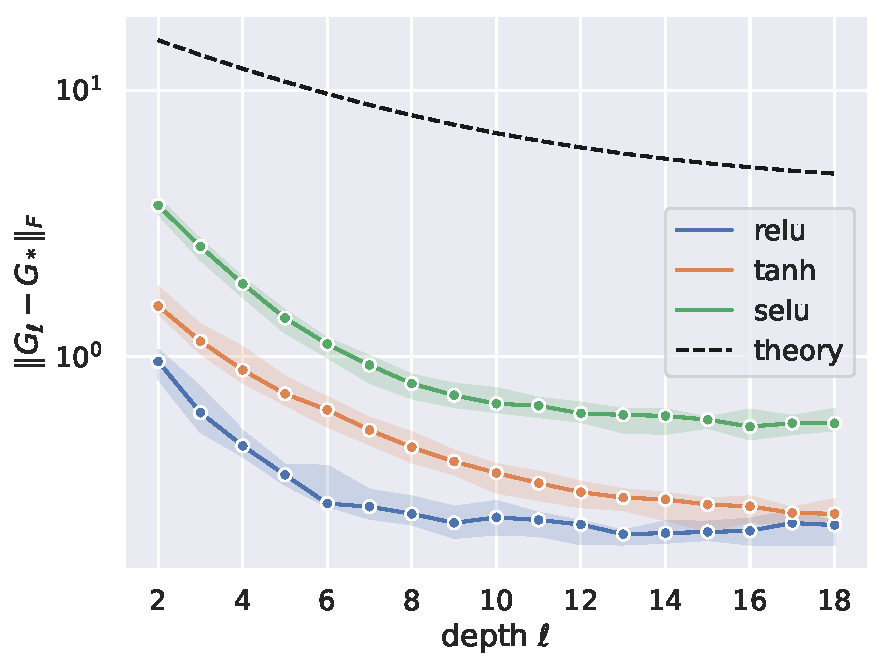
\includegraphics[width=.45\textwidth]{figures/Gram_diff_vs_l.pdf}
\vspace{-.4cm}
\caption{$\|G_\ell - G_*\|_F$ vs. depth, $\ell = 1,2,...,20,$ with a fixed width of $d=1000$ and a batch size of $n=10$. The dashed line shows the theoretical upper bound of Theorem~\ref{MF:thm:concentration}.}
\label{MF:fig:Gram_vs_depth}
\end{figure}
\begin{figure}[ht]
\centering
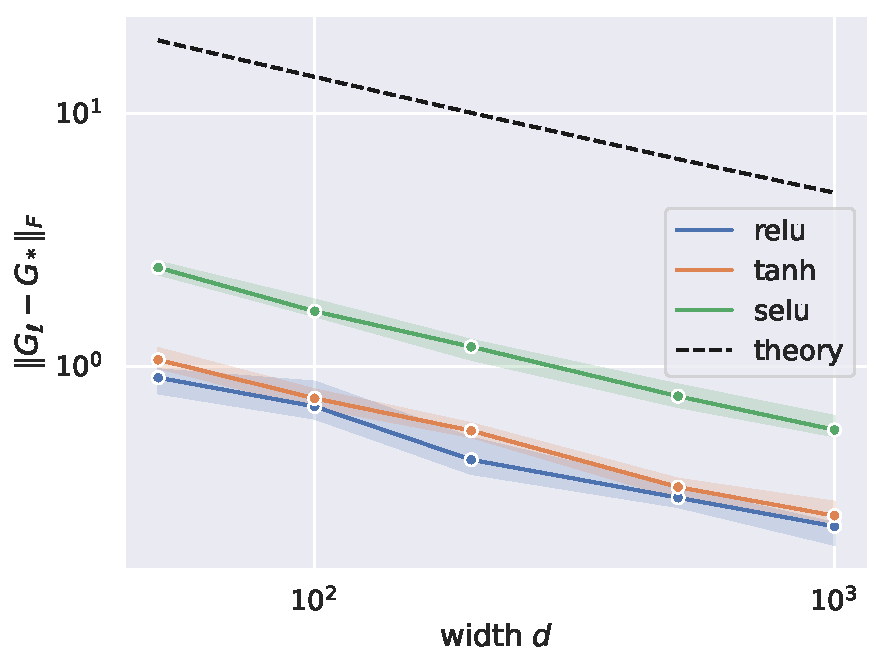
\includegraphics[width=.45\textwidth]{figures/Gram_diff_vs_d.pdf}
\vspace{-.4cm}
\caption{$\|G_\ell - G_*\|_F$ vs. width, $d=50,100,200,500,1000$, with a fixed depth of $\ell=20$ and a batch size of $n=10.$ The second term $O(n/\sqrt{d})$ is always dominant, as demonstrated in the following log-log plot.}
\label{MF:fig:Gram_vs_width}
\end{figure}

\begin{figure}[ht]
\centering
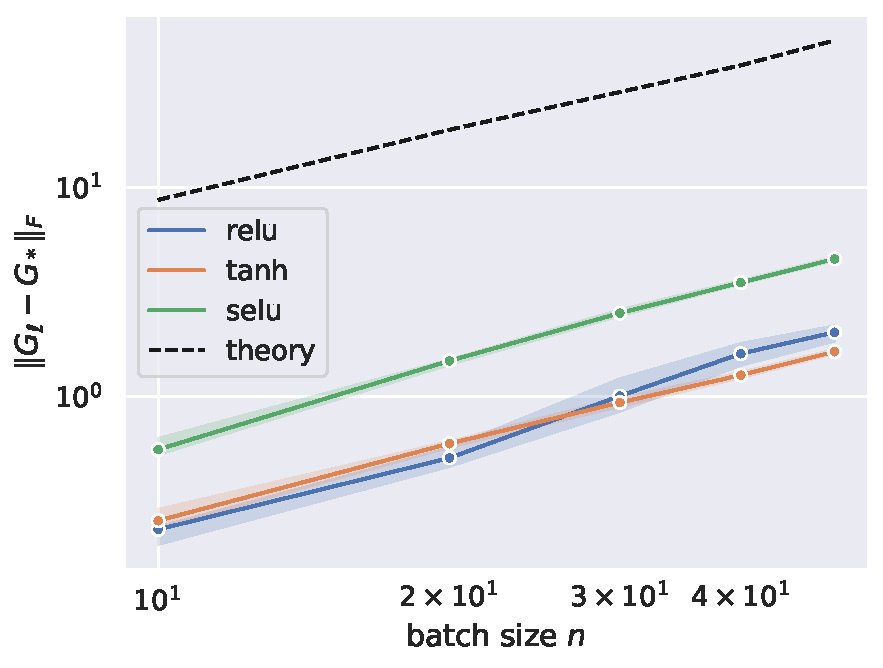
\includegraphics[width=.45\textwidth]{figures/Gram_diff_vs_n.pdf}
\vspace{-.4cm}
\caption{$\|G_\ell - G_*\|_F$ vs. batch size, with a fixed width of $d=1000$ and a depth of $\ell=20,$ and varying batch sizes of $n=10,20,30,40,50.$ Dashed line shows upper bound given in Theorem~\ref{MF:thm:concentration}.}
\label{MF:fig:Gram_vs_n}
\end{figure}

You can find the detailed proofs in Chapter~\ref{ch:bn_MF:proofs}.


% \section{Applications}\label{MF:sec:validations}
% The spectral analysis of Gram matrices plays a central role in numerous theoretical and practical machine learning studies. For instance, these matrices are used to design activations, contributing to improved conditioning~\cite{klambauer2017self}, and to create novel initialization schemes for training convolutional networks with $10000$ layers~\cite{xiao2018dynamical}. One line of research links the enhanced performance of neural networks incorporating batch normalization to the well-conditioning of Gram matrices $G_\ell$ \cite{yang2018a,daneshmand2020batch,daneshmand2021batch}. Since the existing literature often uses mean field approximations, we can leverage Theorem~\ref{MF:thm:concentration} to evaluate accuracy of these approximations for finite width and depth settings.

% \subsection{Well-conditioning with batch normalization}

% Empirical studies suggest that the conditioning of Gram matrices, $G_\ell$, has a substantial impact on the training of deep neural networks \cite{xiao2018dynamical,pennington2018emergence,li2022neural,daneshmand2020batch}. 
% % Observations show that initializing the optimization process from well-conditioned Gram matrices leads to a faster convergence for stochastic gradient descent. 
% Experimental evidence suggests that batch normalization can ensure the good conditioning of $G_\ell$~\cite{yang2018a,daneshmand2021batch}, thereby enhancing the training of deep neural networks.

% In a seminal study, \citet{yang2018a} study the fixed points of the mean field equation of an MLP with batch normalization. In particular, they demonstrate that one fixed point $G_*$ follows the following form:
% \begin{align}\label{MF:eq:stable_G_symmetric}
% \C = b^*\left( (1-c^*)I_n + c^* \1_{n\times n}\right),
% \end{align}
% where $c^*$ and $b^*$ are constants determined by the activation function. Given the distinctive construction for $\C,$ we can deduce the structure of its eigenvalues, with the largest eigenvalue being ${\lambda^*_1=(1+(n-1)c^* )b^*},$ and all others being equal to $\lambda^*_2=\dots=\lambda^*_n = b^*(1-c^*).$ 

% While the mean field analysis discussed above holds for infinitely wide and deep neural networks, it is possible to utilize Theorem~\ref{MF:thm:concentration} to link the spectrum of $\C$ with the spectra of Gram matrices for networks of finite width. Using the Hoffman-Wielandt inequality~\cite{hoffman2003variation}, we can calculate a bound on the deviation of the spectrum of $G_\ell$ from $G_*,$ using the bound on their Frobenius distance.


% \begin{corollary}[Spectral concentration]\label{MF:cor:spectrum}
% In the same settings as Theorem~\ref{MF:thm:concentration}, let $\lambda_i$ and $\lambda_i^*$ denote eigenvalues of $G_\ell$ and $G_*$ respectively in a descending order. Assuming that ${\kappa(G_*) = O(1)}$, the deviation of their spectra $\sqrt{\Sigma_{i=1}^n(\lambda_i-\lambda_i^*)^2}$ is bounded by
% \begin{align}
% O\left((1-\alpha)^{\frac{\ell}{2}}+ \frac{n}{\sqrt{d}}\alpha^{-\frac12}\ln^{\frac12}(\frac{d}{n}) \right),
% \end{align}
% with high probability in $d$ and $\ell.$
% \end{corollary}

% Substituting the spectrum of $\C$ characterized by \citet{yang2018a} into the above concentration, we can estimate the spectra of Gram matrices $G_\ell$, encapsulated in the following proposition.

% \begin{proposition}\label{MF:cor:ESD_spect}
% In the same setting as Theorem~\ref{MF:thm:concentration}, assuming $G_*$ complies with equation~\ref{MF:eq:stable_G_symmetric}, then for a sufficiently deep layer $\ell$, $n-O(1)$ eigenvalues of $G_\ell$ are within $O(\sqrt{n/d})$ range of $b^* (1-c^*)$ with high probability in $d$.
% \end{proposition}

% The above proposition provides a characterization for the ``bulk'' of eigenvalues of~$G_\ell$, by postulating that majority of eigenvalues of $G_\ell$ are concentrated around some absolute constant, up to $\sqrt{n/d}$ range. Interestingly, this bears resemblance to the Marchenko-Pastur~\cite{pastur1967distribution} law on the eigenvalue distribution of Wishart matrices of comparable size. We observe empirically that the singular values of $h_\ell,$ which are square root of eigenvalues of $G_\ell,$ accurately follow the Marchenko-Pastur distribution with $\gamma={n/d}$, as depicted in Figure~\ref{MF:fig:MP_ESD}. Our empirical evaluations show that this distribution accurately predicts singular values of hidden representations for commonly used activation functions with various widths (see Appendix for empirical evidence).

%  \begin{figure}[ht]
%  \centering
%  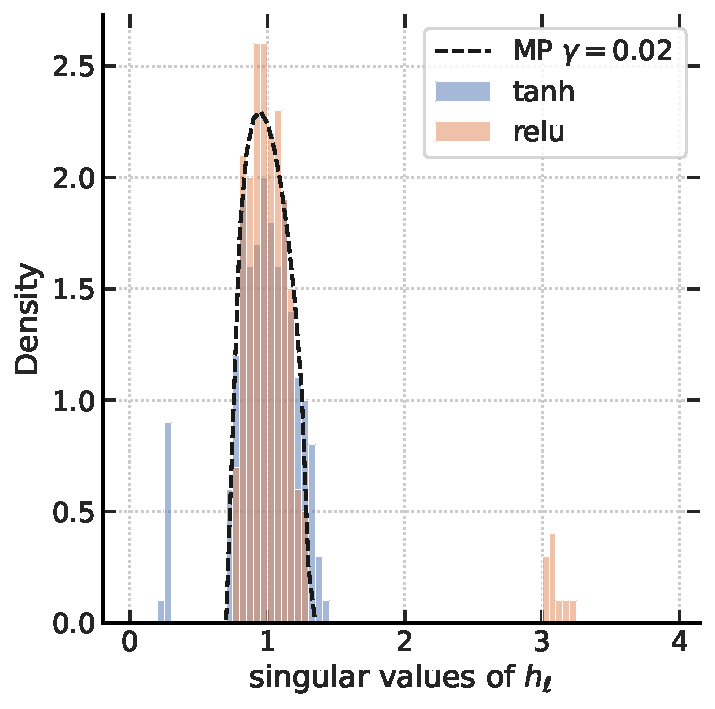
\includegraphics[width=0.4\textwidth]{figures/singular_values_relu_tanh.pdf}
%  \vspace{-.5cm}
%  \caption{BN-MLP with $n=20,d=1000$, $\ell=20$: histogram shows the empirical distribution of singular values of $h_\ell,$ for $\act=\relu$ and $\act=\tanh.$ The black curve marks the Marchenko-Pastur distribution with $\gamma={n/d}=0.02.$ The singular values are normalized by their medians in this plot to be aligned at $1.0$}
%  \label{MF:fig:MP_ESD}
% \end{figure}

% It is worth noting that only the $O(1)$ singular values are influenced by the activation function, while the remaining $n-O(1)$ exhibit a universal behavior. For example in the case of $\act=\relu,$ a single large eigenvalue is associated with the $\1_n$ direction, owing to the non-negativity of $\relu$ outputs. 

% \subsection{Influence of Gram matrix conditioning on training}
% Having explored the influence of batch normalization on the spectra of the Gram matrices, we now turn our attention to its effects during training.  
% It has been hypothesized that batch normalization facilitates the training of neural networks at the initialization stage by ensuring the deep representations are biased towards a uniform prior on class probabilities~\cite{daneshmand2021batch}. In contrast, it has been reported poor Gram matrix conditioning in standard MLP leads to the gradual alignment of deep hidden layers, thereby resulting in highly similar logits across different samples in the batch~\cite{daneshmand2020batch,daneshmand2021batch}. Batch normalization effectively resolves this issue, ensuring a more efficient learning process for the network. While our theoretical studies are limited to initialization, we can empirically explore conditioning of Gram matrix during training. 

% % \paragraph{Gram matrix conditioning during training}
% We examined a standard MLP setup consisting of 10 layers ($L=10$) and a width of 1000 ($d=1000$). We trained this network on mini-batches of size 128 ($n=128$) using the CIFAR100 dataset for 50 epochs, using SGD with a learning rate of $0.001$. This process was carried out on MLP configurations both with and without batch normalization.

% We present the distributions of log-eigenvalues for the penultimate Gram matrix, represented by $\log(\lambda_i(G_L))$, during training in Figure~\ref{MF:fig:training_eigenvals}. It is noteworthy that the eigenvalues of the penultimate Gram matrix for the MLP with batch normalization are more concentrated around their mean than their counterparts in the MLP without batch normalization. This suggests a collapse in class representations in the absence of normalization. 

% To further investigate class representations, we calculated the frequency of each class in the predictions at different training stages. We quantified the entropy of the predicted class probabilities, computed as ${\sum_{i=1}^C p_i \log_2(p_i)}$. In this equation, ${p_c := \frac1N\#\{i\le N: \tilde y_i= c\}}$ designates the proportions of predictions for class $c$, and $\tilde y_i$ represents the prediction for sample $i.$ Observe that a uniform distribution $p_1=\dots = p_C = 1/C,$ leads to the highest entropy $O(\log_2(C))$.

% As illustrated in Figure~\ref{MF:fig:class_entropy}, the MLP with batch normalization closely approximates this uniform prior at initialization. In contrast, the MLP without normalization exhibits a significantly lower initial class entropy. For a balanced dataset like CIFAR100, an optimal model should have a class entropy of approximately $\log_2(100)\approx 6.64$, reflecting a uniform distribution over classes. Hence, batch normalization biases the initial predictions towards a uniform distribution on the labels. The observed discrepancy in Figure~\ref{MF:fig:class_entropy} may thus be related to the accelerated convergence of training loss as depicted in Figure~\ref{MF:fig:training_loss}. 

% The empirical evidence presented here suggests that while Theorem~\ref{MF:thm:concentration} was proven for initialization, Gram matrices of MLP with batch normalization remain well-conditioned during the entire training process. 



% \begin{figure}[ht]
% \centering
% 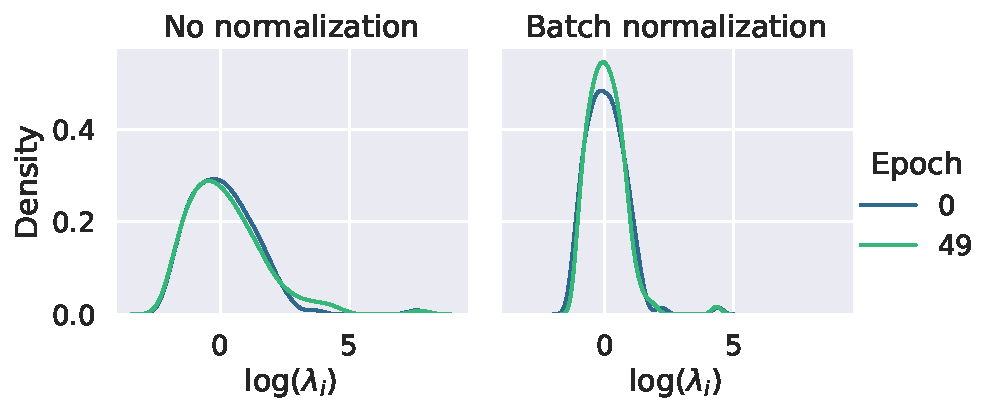
\includegraphics[width=.5\textwidth]{figures/gram_eigenvalues_plot.pdf}
% \vspace{-.8cm}
% \caption{Distribution of log-eigenvalues of penultimate Gram matrix, $\log(\lambda_i(G_L))$ at initialization (epoch $0$) and at the end of training (epoch $49$).}
% \label{MF:fig:training_eigenvals}
% \end{figure}

% \begin{figure}[ht]
% \centering
% 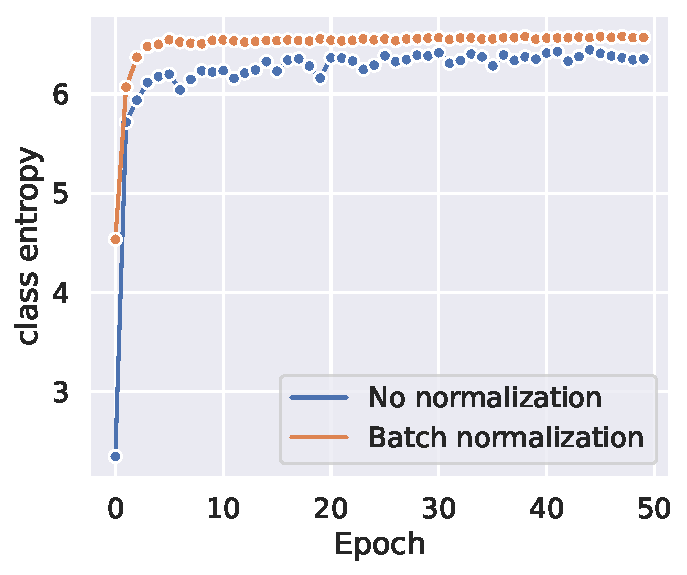
\includegraphics[width=.4\textwidth]{figures/class_entropy.pdf}
% \vspace{-.5cm}
% \caption{Predicted class entropy of MLP with (orange) and without (blue) batch normalization. }
% \label{MF:fig:class_entropy}
% \end{figure}

% \begin{figure}[ht]
% \centering
% 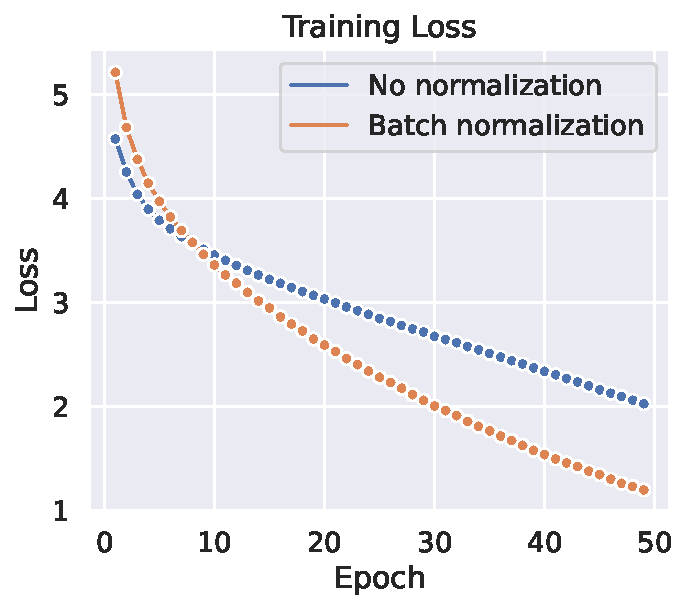
\includegraphics[width=.4\textwidth]{figures/loss_plot.pdf}
% \vspace{-.5cm}
% \caption{Training loss of MLP with (orange) and without (blue) batch normalization on the CIFAR100 dataset.}
% \label{MF:fig:training_loss}
% \end{figure}

\section{Limitations and Future Directions}
In this chapter, we presented a theoretical framework that bridges the gap between the mean field theory of neural networks with finite and infinite widths, with a focus on batch normalization at initialization. Many questions that were out of the scope for this study, suggesting directions for new lines of inquiry. 


\paragraph{Rapidly mixing assumption.}
One limitation of our work is the rapidly mixing assumption that was used to establish the concentration of our results. While our experiments validated our results based on this assumption, it would be beneficial to prove that this assumption holds for a wide range of neural networks with batch normalization.

\paragraph{Training and optimization.}
While our focus of the current work was on random neural networks. In an elegant observation, ~\citet{feng2022rank} demonstrate that the rank of input-output Jacobian of neural networks without normalization at initialization diminishes at an exponential rate with depth (Theorem 5), which implies changes in the input does not change the direction of outputs. In a remarkable observation, ~\citet{yang2018a} show the exact opposite for BN-MLP using a mean field analysis (Theorem 3.10): any slight changes in the input lead to unbounded changes in the output. These results naturally raise the following question: Can we arrive at non-trivial results about input-output Jacobian at the infinite depth finite width regime? 

The mean field approach is also used to analyze the training mechanism. In particular,~\citet{bach2021gradient} prove that gradient descent globally converges when optimizing single-layer neural networks in the limit of an infinite number of neurons. Although the global convergence does not hold for standard neural networks, insights from this mean field analysis can be leveraged in understanding the training mechanism.  

\paragraph{Exploring other normalizations.}
More research is needed for other normalization techniques, such as weight normalization~\cite{salimans2016weight} or layer normalization~\cite{ba2016layer} to understand the impact of these normalization techniques on the robustness and generalization of neural networks. Our findings highlight the power of mean field theory for analyzing neual networks with normalization layers.

\paragraph{Extending to other architectures}
Our analyses are limited to MLPs. Extending our work to convolutional neural networks and transformers would enable us to analyze and enhance initialization for these neural networks. In particular, recent studies have shown that transformers suffer from the rank collapse issue when they grow in depth~\cite{anagnostidissignal}. A non-asymptotic mean field theory may enable us to tackle this issue by providing a sound understanding of representation dynamics in transformers.

Overall, our results demonstrate that depth is not necessarily a curse for mean field theory, but can even be a blessing when neural networks have batch normalization. The inductive bias provided by batch normalization controls the error propagation of mean field approximations, enabling us to establish non-asymptotic concentration bounds for mean field predictions. This result underlines the power of mean field analyses in understanding the behavior of deep neural networks, thereby motivating the principle development of new initialization and optimization techniques for neural networks based on mean field predictions. 


